\section{System Analysis: architecturally significant requirements}
\label{sec:analysis_requirements}
In the section at hand, we report the findings of the top-down analysis of the Apache MINA framework. We perform a thorough investigation of various sources, as described in section \ref{sec:overview_of_sources}, without considering the codebase of the project, in order to distil the core functionalities of the MINA (see section \ref{sec:features}) and the significant quality attributes (see section \ref{sec:quality_attributes}), which are key drivers for the architecture of the project.

\subsection{Overview of sources}
\label{sec:overview_of_sources}
For the top-down analysis, we use the following sources:
\begin{enumerate}
    \item Official website \cite{mina-website}
    \item Documentation \cite{mina-docs}
    \begin{enumerate}
        \item Presentations \cite{mina-talk2006, mina-talk2008}
        \item User guide \cite{mina-userguide}
        \item Tutorials (Quick Start guide) \cite{mina-qsguide}
    \end{enumerate}
    \item API documentation \cite{mina-reference} \footnote{This will mostly be of help for determining the architectural components}
    \item User testimonials \cite{mina-testimonials}
\end{enumerate}
The User guide includes various tutorials that will aid us in understanding the full extent of the project's functionalities. The User testimonials are an informal source, however we believe it will strengthen the validation of the quality attributes.

The information significant for the understanding of the requirements of the project is annotated and presented in this section to support and validate our analysis. We present excerpts from the sources with their corresponding links that can be easily checked.

\subsection{System's features}
\label{sec:features}
Researching the official documentation, the features offered by MINA immediately become apparent. An overview of the features is presented in figure \ref{fig:features}, as extracted from the documentation \cite{mina-docs}. Most of these features correspond to the functional requirements of the framework. We identify the following 2 core architecturally significant functional requirements, as distilled from these features and complementary sources:
\begin{itemize}
    \item Provide a layer of abstraction on top of the networking layer, which hides the differences between Blocking and Non-blocking IO, which simulates a blocking mode. This enables the development of network applications which, in essence, consist of a server and a client side communicating over some network protocol (e.g. TCP, UDP). 
    
    \source{[...] the best solution is to hide this aspect by writing a framework that mimics a blocking mode. This is what MINA does!}{\cite[Sec. 1.2]{mina-userguide}}
    
    \item Standardize the IO application vision w.r.t. transport types (e.g. TCP/IP, UDP/IP, serial and in-VM pipe  communication, custom).
    
    \source{It provides a common IO vision to an application that needs to communicate over TCP, UDP or whatever mechanism. [...] MINA does not only handle TCP and UDP, it also offers a layer on top of serial communication (RSC232), over VmpPipe or APR.}{\cite[Sec. 1.2]{mina-userguide}}
\end{itemize}

\begin{figure}
    \centering
    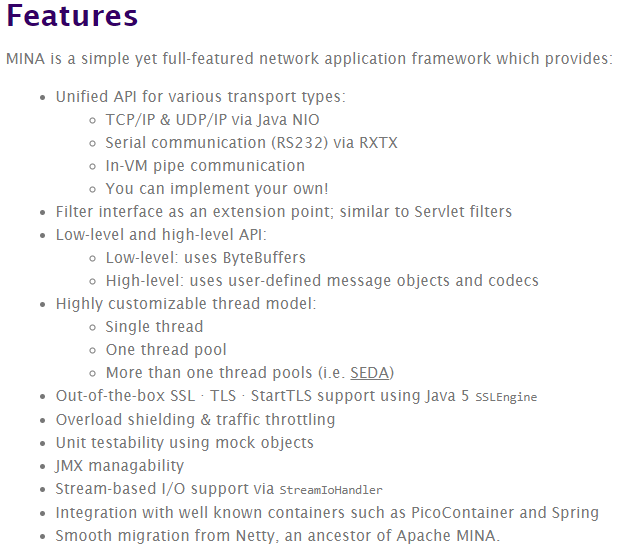
\includegraphics[width=0.7\textwidth]{images/features.png}
    \caption{An overview of the features provided by Apache MINA extracted from the official documentation.}
    \label{fig:features}
\end{figure}

The core feature of the framework is, therefore, the \textit{Unified API for various transport types}. The remaining features mentioned in figure \ref{fig:features} are additions to the core MINA project that not only extend the functionality of the framework, but, most importantly, ensure the expected quality attributes discussed below.

\subsection{Quality attributes}
\label{sec:quality_attributes}

\source{Apache MINA is a network application framework which helps users develop high performance and high scalability network applications easily.}{\cite{mina-website}}

From this definition of Apache MINA on the official website it follows that the key drivers of the project are \textit{performance} and \textit{scalability}. We have further identified other significant quality attributes of the framework itself, as well as the MINA based applications, which are individually explored below and correlated to the features or functionalities through which these qualities are achieved.

\subsubsection{Performance \& scalability}
MINA has been specifically designed to work both on the client and server side, performance and scalability therefore being of paramount importance for adapting to server requirements. In terms of design decisions, NIO communication has been chosen as the building block of MINA since it offers better scalability for a large number of connections (i.e. over a few thousands). The performance of the framework has been tested over AMQP (Advanced Message Queuing Protocol), the results are showcased in the introductory presentation \cite{mina-talk2006}. As an example, MINA offers \textit{overload shielding \& traffic throttling} to ensure these qualities.

\source{Writing a server makes it critical to have a scalable system, which is tunable to fit the server needs, in terms of performance and memory usage. This is what MINA is good for, making it easy to develop you server.}{\cite[Sec. 1.2]{mina-userguide}}

\source{This is true for up to a few thousands of connected users, but up to a point, the BIO approach just stops scaling; you won’t be able to handle millions of connected users using one thread per user! NIO can. Now, one other aspect is that the time spent in the MINA part of your code is probably non significant, ...}{\cite[Sec. 1.2]{mina-userguide}}


\subsubsection{Usability}
Programming network application has a stigma of being regarded as low level programming and a highly complicated task. MINA comes as a response and provides a user friendly framework. This is achieved through the various features which allow for high degrees of user customization: own implementation of transport types, high-level API with user defined message objects, customizable thread model (see figure \ref{fig:features}). Moreover, the extensive documentation sources (user guide, tutorials etc.) aid the user in the implementation of their own applications on top of MINA.

\source{Ease of use When you have no special performance requirements, MINA is probably a good choice as it allows you to develop a server or a client easily [...] You could probably write your server with only a few lines of code...}{\cite[Sec. 1.2]{mina-userguide}}

\source{You just have to design your application on top of MINA without having to handle all the complexity of the newtork layer.}{\cite[Sec. 2.1]{mina-userguide}}

\source{This gives you the ease of mind that you won’t have to spend hours on some cryptic errors in your own implementation of the network layer.}{\cite[Sec. 1.2]{mina-userguide}}

\source*{Figure \ref{fig:usability_extensibility} shows the ease of use of the framework in creating network applications (i.e. a simple echo server).}


\subsubsection{Testability}
The unified API offered by MINA follows an abstract design approach; this supports unit tests. As seen in figure \ref{fig:features}, the framework is unit test friendly and also provides mock objects to increase the testability of the applications developed on top of MINA.

\source{Unit-testable, abstract API, out-of-the-box mock objects}{\cite[p.6]{mina-talk2008}}

\subsubsection{Extensibility}
%run time extensible through filters
Applications built on top of MINA can be easily extended. This is implemented through the filters feature (see figure \ref{fig:features}). The filters can modify the application behaviour at runtime (e.g. logging filter, blacklist remote address filter); the filters are dynamically activated which provides additional flexibility for the MINA based applications. Figure \ref{fig:filters} shows an overview of the out-of-the-box filters included in the framework. As an advanced topic, users can configure their own IO filters, which reinstates the high customization degree of the framework.

\source{Extensible, Runtime modification of application behavior using `filters'.}{\cite[p.7]{mina-talk2008}}

\source{Many out-of-the-box filters are provided to accelerate network application development pace by simplifying typical cross-cutting concerns using the out-of-the-box filters.}{\cite[Sec. 5]{mina-userguide}}

\source*{Figure \ref{fig:usability_extensibility} presents options for extending the functionality of a simple server application.}

\subsubsection{Maintainability \& reusability}
MINA has been designed with the maintainability and reusability concerns in mind; this is immediately apparent when considering the high-level architecture of the framework. A high-level overview is presented in figure \ref{fig:architecture}. A more in depth account of the architectural components is presented in section \ref{sec:analysis_components}. For now, we foucs on the layered structure which enforces separation of concerns: the business logic is completely separated from the processing of the IO. Moreover, at the IO Service and Filter Chain levels, out-of-the-box components are provided, allowing the user to focus mainly on the application layer which involves the logic of handling the messages. The separation of concerns involved with the architecture design, together with the variety of pre-made components, enforce the maintainability and reusability of MINA.

\source{Broadly, MINA based applications are divided into 3 layers: \begin{itemize*}\item I/O Service - Performs actual I/O \item I/O Filter Chain - Filters/Transforms bytes into desired Data Structures and vice-versa \item I/O Handler - Here resides the actual business logic \end{itemize*}}{\cite[Sec. 2.1]{mina-userguide}}

\source*{Figure \ref{fig:reusability} showcases the modular and reusable nature of components which build the MINA architecture.}

\begin{figure}
    \centering
    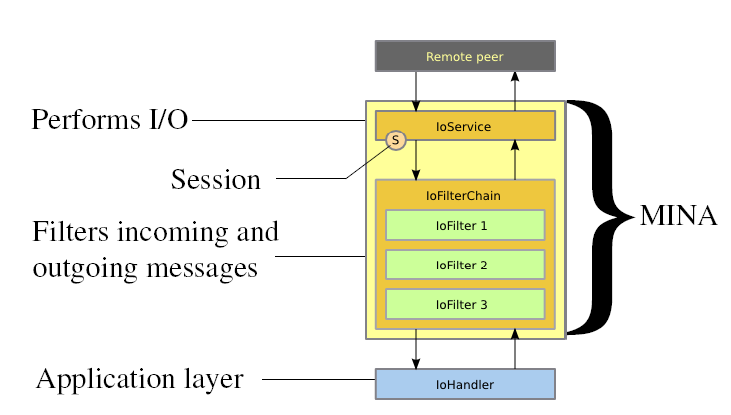
\includegraphics[width=\textwidth]{images/architectural_overview.png}
    \caption{MINA architectural overview as presented in the presentation "MINA in Real Life (ApacheCon EU 2009)".}
    \label{fig:architecture}
\end{figure}




\subsubsection{Stability}
MINA is a proven system with a stable architecture; it is presently used by various applications, therefore a drastic structural change is unlikely. None the less, MINA has had a stable evolution empowered by the component modularity of its architecture: the core of the architecture remained stable, while components have been added to extend the functionality of the framework (e.g. the filters functionality mentioned above). The sustained effort of maintaining the framework and its documentation (especially the API design) also contributes to its stability.

\source{A proven system MINA is used by many applications all over the world. There are some Apache projects based on MINA, and they are working pretty well.}{\cite[Sec. 1.2]{mina-userguide}}

\subsubsection{Integration \& manageability}
MINA offers integration with a number of third-part systems (e.g. PicoContainer, Spring) among which JMX (Java Management Extensions, see figure \ref{fig:features}). Through connection with the JMX API, the management of MINA based applications is facilitated.

\source{Java Management Extensions (JMX) is used for managing and monitoring java applications. This tutorial will provide you with an example as to how you can JMX-enable your MINA based application.}{\cite[Sec. 16]{mina-userguide}}

\source*{Figure \ref{fig:manageability} presents the added management functionality provided through the JMX integration.}
\subsection{Quality attributes validation}
Quality attributes pertain to non-functional requirements of a system. They can span the entire system and are difficult to quantify. Since non-functional qualities of a system are closely related to the user's needs and expectations of the system, we present a series of user informal evaluations of MINA in order to validate its quality attributes; these evaluations are extracted from \cite{mina-testimonials}.

\begin{itemize}
    \item \textsc{Performance, Scalability, Maintainability}: \textit{``I found that Apache MINA really did fulfill its promise and implementing a high-performance, scalable and extensible network server was easy using it. MINA also helps very cleanly separate network communication and application level message processing logic.''} 
    \item \textsc{Performance, Stability, Usability}: \textit{``We found the speed and stability of MINA to be excellent. And although we are still using MINA 0.8.1, we found the API very elegant and easy.''}
    \item \textsc{Performance, Stability, Testability}: \textit{``[...]MINA was a real treat as it saved a lot of time, is well written and gets more testing than our in house QA would be able to cover. The speed and stability of our app on top of MINA has been excellent.''}
    \item \textsc{Usability}: \textit{``[...]It makes writing server applications simple and is much easier to use than Java’s NIO libraries. Because of MINA’s stability and ease of use, we plan on using MINA more in our future projects.''}
\end{itemize}